% This file was created with tikzplotlib v0.9.17.
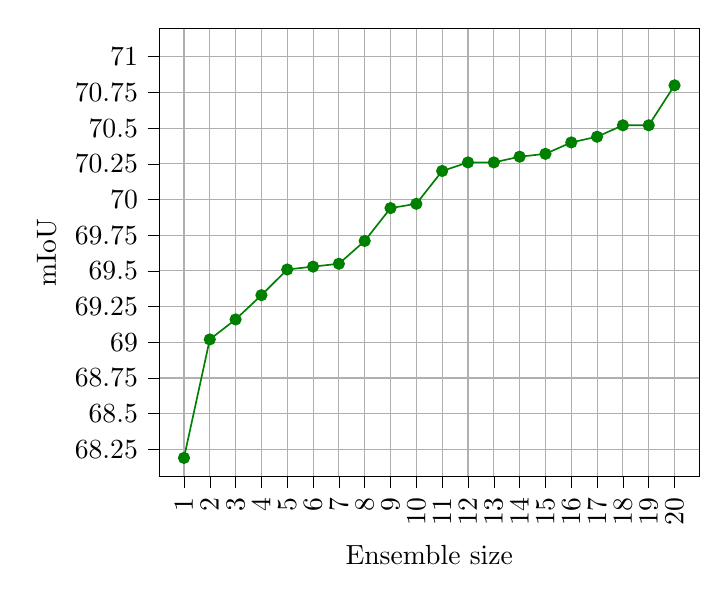
\begin{tikzpicture}

\begin{axis}[
tick align=outside,
tick pos=left,
x grid style={white!69.0196078431373!black},
xlabel={Ensemble size},
xmajorgrids,
xmin=0.0499999999999999, xmax=20.95,
xtick style={color=black},
xticklabel style={rotate=90},
xtick={1, 2, 3, 4, 5, 6, 7, 8, 9, 10, 11, 12, 13, 14, 15, 16, 17, 18, 19, 20},
y grid style={white!69.0196078431373!black},
ylabel={mIoU},
ymajorgrids,
ymin=68.0595, ymax=71.2,
ytick={68.25, 68.5,68.75, 69, 69.25, 69.5, 69.75, 70,70.25, 70.5, 70.75, 71},
ytick style={color=black}
]
\addplot [draw=green!50!black, fill=green!50!black, mark=*, only marks]
table{%
x  y
1 68.19
2 69.02
3 69.16
4 69.33
5 69.51
6 69.53
7 69.55
8 69.71
9 69.94
10 69.97
11 70.2
12 70.26
13 70.26
14 70.3
15 70.32
16 70.4
17 70.44
18 70.52
19 70.52
20 70.8
};
\addplot [semithick, green!50!black]
table {%
1 68.19
2 69.02
3 69.16
4 69.33
5 69.51
6 69.53
7 69.55
8 69.71
9 69.94
10 69.97
11 70.2
12 70.26
13 70.26
14 70.3
15 70.32
16 70.4
17 70.44
18 70.52
19 70.52
20 70.8
};
\end{axis}

\end{tikzpicture}
